%-------------------------------------------------------------------------------
% ABSOLVENTSKÁ PÍSEMNÁ PRÁCE
% TeX, verze 03-2022
%-------------------------------------------------------------------------------

%-------------------------------------------------------------------------------
% KONFIGURACE PRÁCE
%-------------------------------------------------------------------------------

% metadata práce
% ------------------------------------------------------------------------------
% PROMĚNNÉ PROSTŘEDÍ
% ------------------------------------------------------------------------------

% jméno autora práce
\newcommand{\autor}{Josef Novák}

% prohlášení - tvar vypracoval/vypracovala
\newcommand{\osoba}{vypracoval/a}

% studijní obor a program
\newcommand{\studijniObor}{Hudba/Zpěv}
% pro obor zpěv ponechte program prázdný (~)
\newcommand{\studijniProgram}{Hra na nástroj}

% téma absolventské písemné práce
\newcommand{\appTema}{Název\\ absolventské práce}

% vedoucí práce a vyučující hlavního oboru
\newcommand{\appVedouci}{Mgr.~Jiří Vedoucí}
\newcommand{\appUcitel}{MgA.~Pavel Hráč}

% škola a místo
\newcommand{\skola}{Konzervatoř Pardubice}
\newcommand{\misto}{Pardubice}

% rok odevzdání/obhajoby APP
\newcommand{\skolniRok}{\the\year{}}

% datum odevzdání - pro datum překladu do PDF \today
\newcommand{\datumOdevzdani}{\today}

% "Shrnutí" v cizím jazyce
\newcommand{\shrnutiCizi}{Summary} % Angličtina
%\newcommand{\shrnutiCizi}{Zusammenfassung} % Němčina

% "Klíčová slova" v cizím jazyce
\newcommand{\klicovaSlovaCiziLit}{Keywords} % Angličtina
%\newcommand{\klicovaSlovaCiziLit}{Schlüsselwörter} % Němčina

% klíčová slova CZ
\newcommand{\klicovaslova}{slovo1, slovo2, slovo3, slovo4, slovo5}
% klíčová slova v cizím jazyce
\newcommand{\klicovaslovaCizi}{word1, word2, word3, word4, word5}


% základní konfigurace a balíčky
%%%%%%%%%%%%%%%%%%%%%%%%%%%%%%%%%%%%%%%%%%%%%%%%%%%%%%%%%%%%%%%%%%%%%%%%%%%%%%%%

% metadata práce
% ------------------------------------------------------------------------------
% PROMĚNNÉ PROSTŘEDÍ
% ------------------------------------------------------------------------------

% jméno autora práce
\newcommand{\autor}{Josef Novák}

% prohlášení - tvar vypracoval/vypracovala
\newcommand{\osoba}{vypracoval/a}

% studijní obor a program
\newcommand{\studijniObor}{Hudba/Zpěv}
% pro obor zpěv ponechte program prázdný (~)
\newcommand{\studijniProgram}{Hra na nástroj}

% téma absolventské písemné práce
\newcommand{\appTema}{Název\\ absolventské práce}

% vedoucí práce a vyučující hlavního oboru
\newcommand{\appVedouci}{Mgr.~Jiří Vedoucí}
\newcommand{\appUcitel}{MgA.~Pavel Hráč}

% škola a místo
\newcommand{\skola}{Konzervatoř Pardubice}
\newcommand{\misto}{Pardubice}

% rok odevzdání/obhajoby APP
\newcommand{\skolniRok}{\the\year{}}

% datum odevzdání - pro datum překladu do PDF \today
\newcommand{\datumOdevzdani}{\today}

% "Shrnutí" v cizím jazyce
\newcommand{\shrnutiCizi}{Summary} % Angličtina
%\newcommand{\shrnutiCizi}{Zusammenfassung} % Němčina

% "Klíčová slova" v cizím jazyce
\newcommand{\klicovaSlovaCiziLit}{Keywords} % Angličtina
%\newcommand{\klicovaSlovaCiziLit}{Schlüsselwörter} % Němčina

% klíčová slova CZ
\newcommand{\klicovaslova}{slovo1, slovo2, slovo3, slovo4, slovo5}
% klíčová slova v cizím jazyce
\newcommand{\klicovaslovaCizi}{word1, word2, word3, word4, word5}


%%%%%%%%%%%%%%%%%%%%%%%%%%%%%%%%%%%%%%%%%%%%%%%%%%%%%%%%%%%%%%%%%%%%%%%%%%%%%%%%

\renewcommand{\baselinestretch}{1.2}

\usepackage{pdfpages} % vnoření PDF
\usepackage{newclude}

\usepackage[main=czech]{babel} % čeština
\usepackage{csquotes} % české uvozovky

%%%%%%%%%%%%%%%%%%%%%%%%%%%%%%%%%%%%%%%%%%%%%%%%%%%%%%%%%%%%%%%%%%%%%%%%%%%%%%%%
% LITERATURA A REFERENCE
%%%%%%%%%%%%%%%%%%%%%%%%%%%%%%%%%%%%%%%%%%%%%%%%%%%%%%%%%%%%%%%%%%%%%%%%%%%%%%%%

% literatura - ISO 690
\usepackage[
   backend=biber
  ,style=iso-numeric
  ,sortlocale=cs_CZ
  ,sorting=nyt
  ,maxnames=3
  ,minnames=3
  ,pagetotal=true
  ,autolang=other
  ,bibencoding=UTF8
  ,spacecolon=false % mezera před dvojtečkou
]{biblatex}

\setcounter{biburllcpenalty}{7000}
\setcounter{biburlucpenalty}{8000}

\addbibresource{./literatura.bib}

% formátování seznamu zdrojů a literatury
\DeclareFieldFormat{labelnumberwidth}{[\,{#1}\,]}
\defbibenvironment{bibliography}
  {\list
     {\printtext[labelnumberwidth]{%
        %%\printfield{prefixnumber}%
        \printfield{labelprefix}%
        \printfield{labelnumber}}}
     {\setlength{\labelwidth}{\labelnumberwidth}%
      \setlength{\leftmargin}{\labelwidth}%
      \setlength{\labelsep}{\biblabelsep}%
      \addtolength{\leftmargin}{+1.5\labelsep}%
      \setlength{\itemsep}{\bibitemsep}%
      \setlength{\parsep}{\bibparsep}}%
      \renewcommand*{\makelabel}[1]{\hss##1}}
  {\endlist}
  {\item}

%%%%%%%%%%%%%%%%%%%%%%%%%%%%%%%%%%%%%%%%%%%%%%%%%%%%%%%%%%%%%%%%%%%%%%%%%%%%%%%%

% přílohy
\usepackage[titletoc]{appendix}

% tabulky a poznámky pod čarou
\usepackage{tabularx}
\usepackage{makecell}
\usepackage{footnote}

% obrázky v textu
\usepackage{wrapfig}
\usepackage{subcaption}

% matematické prostředí
\usepackage{amsmath}
\usepackage{mathtools}

% stojatá řecká písmena
\usepackage{upgreek}

% rámečky
\usepackage{framed}

% barvy
\usepackage{xcolor}

% formátování a záhlaví
\usepackage{xunicode,xltxtra,url,parskip}
\setlength{\parindent}{1cm}
\usepackage{fancyhdr}

% kreslení v TikZ
\usepackage{tikz,pgfplots}
\pgfplotsset{compat=1.18}
\usepackage[simplified]{pgf-umlcd}
\usepgfplotslibrary{polar}
\tikzset{fontscale/.style = {font=\relscale{#1}}}
\usepackage[siunitx,european]{circuitikz} % evropské značky, jednotky SI
\usetikzlibrary{intersections}

% úprava nadpisů a řádkování
\usepackage{titlesec}
\usepackage{setspace}

% změna záhlaví, hypertextové odkazy bez rámečků
\usepackage{chngcntr}
\usepackage[hidelinks]{hyperref}
\hypersetup{
	colorlinks=false,
	pdfborder={0 0 0},
}

% ovládání software, klávesnice
\usepackage{menukeys}

% vložené zdrojové kódy
\usepackage{verbatimbox}

\makeatletter
\newcommand\verbfilelist[2][]{%
  \setcounter{VerbboxLineNo}{0}%
  \def\verbatim@processline{%
    {\addtocounter{VerbboxLineNo}{1}%
    #1\setbox0=\hbox{#1\the\verbatim@line}%
    \hsize=\wd0 \the\verbatim@line\par}}%
  \verbatiminput{#2}
  \let\verbatim@processline\sv@verbatim@processline
}
\makeatother

%%% STRÁNKA A KAPITOLY %%%%%%%%%%%%%%%%%%%%%%%%%%%%%%%%%%%%%%%%%%%%%%%%%%%%%%%%%

% okraje stránky
\usepackage[
  top=25mm,
  bottom=25mm,
  left=40mm,
  right=25mm,
  %includehead,
  includefoot,
  heightrounded, % underfull zarovnání
]{geometry}

%\renewcommand*\thechapter{\arabic{chapter}}

% číslování obrázků
\counterwithin{figure}{chapter}

% čísla rovnic pod kapitolou a pod podkapitolou
\counterwithin*{equation}{chapter}
\counterwithin*{equation}{section}

% čísla tabulek
\counterwithin{table}{section}

% nadpis kapitoly
\titleformat{\chapter}{\bf\raggedright\Large}{\thechapter.~}{0em}{}
\titlespacing{\chapter}{0pt}{3pt}{3pt}

% podnadpis
%\titleformat{\section}{\bf\raggedright\large}{\thechapter.\thesection.~}{0em}{}
\titlespacing{\section}{0pt}{3pt}{3pt}

% podpodnadpis
%\titleformat{\subsection}{\bf\raggedright}{\thechapter.\thesubsection.~}{0em}{}

% podpodnadpis
%\titleformat{\subsubsection}{\bf\raggedright}{\thesubsubsection.~}{0em}{}
%\titlespacing{\subsubsection}{0pt}{3pt}{3pt}

% příkazy
\newcommand{\nadpis}[1]{
    \chapter{#1}
}

\newcommand{\podnadpis}[1]{
    \section{#1}
}

\newcommand{\podpodnadpis}[1]{
    \subsection{#1}
}

% kapitola vždy začíná na nové stránce
%\AddToHook{cmd/section/before}{\clearpage}

% výchozí záhlaví a zápatí stránky
\lhead{}
\rhead{}
\cfoot{}

% základní styl
\fancypagestyle{StyleBase} {
	\fancyhf{}
	\lhead{}
	\rhead{}
	\cfoot{\thepage}
	\rfoot{}
}

% styl příloh
\fancypagestyle{StyleAppendix} {
	\fancyhf{}
	\lhead{}
	\rhead{}
	\cfoot{\thepage}
	\rfoot{Přílohy}
}

% prázdná stránka
\fancypagestyle{StyleBlank} {
	\fancyhf{}
	\lhead{}
	\rhead{}
	\cfoot{}
	\rfoot{}
	\renewcommand{\headrulewidth}{0pt}
}

%%% VLASTNÍ PŘÍKAZY %%%%%%%%%%%%%%%%%%%%%%%%%%%%%%%%%%%%%%%%%%%%%%%%%%%%%%%%%%%%

% tečkovaná vodící čára pro podpisy
\newcommand{\dotrule}[1]{%
   \parbox[t]{#1}{\dotfill}}

% nadpis bez čísel
\newcommand{\nadpisBezCisla}[1]{
	\newpage
    \setcounter{chapter}{0}
    \setcounter{section}{0}
    \chapter*{#1}
    \addcontentsline{toc}{chapter}{#1}
}

% dvojité podtržení
\def\doubleunderline#1{\underline{\underline{#1}}}

% nota - tón
\newcommand\note[1]{\xnote#1\relax\relax\relax}
	\def\xnote#1#2#3\relax{#1\if#2\relax\else\if b#2$\flat\if#3\relax%
	\else_{#3}\fi$\else\if###2$\sharp\if#3\relax\else_{#3}\fi$\else$_{#2}$\fi\fi\fi}

% záporná nota
\def\noteminus{%
  \setbox0=\hbox{-}%
  \vcenter{%
    \hrule width\wd0 height \the\fontdimen8\textfont3%
  }%
}

% volná, nečíslovaná stránka
\newcommand\blankpage{%
    \null
    \clearpage
    \thispagestyle{empty}%
    %\addtocounter{page}{-1}%
    \newpage
    \clearpage}

\newlength\longest

%%%%%%%%%%%%%%%%%%%%%%%%%%%%%%%%%%%%%%%%%%%%%%%%%%%%%%%%%%%%%%%%%%%%%%%%%%%%%%%%

% slovník
% slovník pro korektní zalamování slov

% en
\hyphenation{Lily-Pond}
\hyphenation{Muse-Score}


% PDF metadata
\author{\autor}
\hypersetup
{
    pdfauthor={\autor},
    pdfsubject={Absolventská písemná práce {\skolniRok}},
    pdftitle={\appTema}
}



%-------------------------------------------------------------------------------
% ZAČÁTEK DOKUMENTU
%-------------------------------------------------------------------------------

\begin{document}

%-------------------------------------------------------------------------------
% TITULNÍ LIST
%-------------------------------------------------------------------------------

% titulní list

\pagestyle{empty}

\begin{center}

	\begin{Large}
		\noindent
		{\textbf{\MakeUppercase{\skola}}}
	\end{Large}

	\vfill

	\begin{Large}
		\noindent
		Absolventská práce
	\end{Large}

	\begin{spacing}{1.8}
		\begin{huge}
			\noindent
			\textbf{\MakeUppercase{\appTema}}
		\end{huge}
	\end{spacing}

	\vfill

	\begin{Large}
		\noindent
		\textbf{\autor}
	\end{Large}


	\begin{large}
		\noindent
		Obor: {\studijniObor}

		\noindent
		{\studijniProgram}
	\end{large}

\end{center}

\vfill

\begin{large}
	\begin{tabularx}{\textwidth}{ l X }
		Vedoucí práce:	& {\appVedouci} \\
		Pedagog hlavního oboru:	& {\appUcitel} \\
	\end{tabularx}
\end{large}

\vfill

\begin{center}
	\begin{large}
		\noindent
		\textbf{\MakeUppercase{\misto}}

		\noindent
		\textbf{\MakeUppercase{\skolniRok}}
	\end{large}
\end{center}

\newpage


%-------------------------------------------------------------------------------
% PROHLÁŠENÍ O SAMOSTATNOSTI
%-------------------------------------------------------------------------------

% prohlášení o samostatnosti

\pagestyle{empty}

{~}
\vfill

\noindent
Čestně prohlašuji, že jsem absolventskou práci {\osoba} samostatně \\
s~použitím uvedených pramenů a~literatury.

\vfill

\begin{spacing}{1.2}
\noindent
\begin{tabularx}{\textwidth}{ X c }
   V~Pardubicích     & \dotrule{3.5cm} \\
   {\datumOdevzdani} & {\autor} \\
\end{tabularx}
\end{spacing}

\newpage


%-------------------------------------------------------------------------------
% PODĚKOVÁNÍ (nepovinné)
%-------------------------------------------------------------------------------

% poděkování

\pagestyle{empty}

{~}
\vfill

\noindent
List s~textem poděkování není povinný a~lze jej vynechat zakomentováním vstupu
v~souboru \texttt{app.tex}.

\newpage


%-------------------------------------------------------------------------------
% OBSAH A SEZNAM PŘÍLOH
%-------------------------------------------------------------------------------

\setcounter{tocdepth}{3}

% obsah
\addtocontents{toc}{\protect\thispagestyle{empty}}
\tableofcontents

% samostatný seznam příloh na nové straně
\newpage
\addtocontents{apc}{\protect\thispagestyle{empty}}
\listofappendix

%-------------------------------------------------------------------------------
% VLASTNÍ TEXT PRÁCE
%-------------------------------------------------------------------------------

\clearpage
\pagestyle{StyleBase}

% Úvod -------------------------------------------------------------------------
\nadpisBezCisla{Úvod}
\setcounter{page}{1}
Úvod předkládá metodologickou a~koncepční charakteristiku práce. Nepovinně může
začínat autorovou motivací k~napsání dané práce, ovšem stejně jako samostatný
text by i~motivace měla být psána v~minulém čase trpného rodu a~bez výrazného
citového zabarvení.

V~úvodu musí dojít k~vymezení tématu (z~hlediska teritoriálního,
časového,\dots) a~jeho zařazení ve~stěžejních dobových reáliích. Tedy: \textit{
Co bude práce zkoumat a~co už ne. A~proč.} Dále musí být stanoveny hlavní cíle
práce - co chce práce vyřešit, objasnit, jakou otázku si klade za~cíl
zodpovědět, k~jakému konkrétnímu cíli chce dospět, a~uvedeny skutečnosti, které
naopak nebudou v~rámci daného tématu zkoumány, ať už z~důvodu rozsahu práce, či
jiných.

Úvod by měl také shrnovat, jakými metodami bude realizováno splnění vytyčených
cílů (např.~analýza, syntéza, srovnání, apod.). Nepovinně též může zahrnovat
vymezení použité terminologie, pokud bude práce specifické terminologie
potřebovat.

\podnadpisBezCisla{Stav bádání}
Stav bádání (angl. \textit{state-of-art}; spíše pouze pokud je tak rozsáhlý, že
skutečně vyžaduje samostatnou kapitolu umístěnou ihned po~Úvodu) shrnuje
a~kriticky rozebírá odbornou literaturu a~dostupné prameny vztahující se
ke~zvolenému tématu.

% Práce ------------------------------------------------------------------------

\nadpis{Šablona a~formální požadavky APP}
Kompletní požadavky k~absolventským písemným pracím shrnuje směrnice
Konzervatoře Pardubice č.~5/19, jejíž plné znění je k~dispozici na webových
stránkách školy v~nabídce \textit{Studium – Absolutorium}.
 
Šablona si klade za cíl zjednodušit formální stránku práce, aby měli autoři
více času na samotný obsah.


Nadpisy první úrovně automaticky začínají na nové straně.
Použití citace.~\cite{harry}


\podnadpis{Doporučená minimální struktura práce}
Základní struktura absolventské práce udává zejména závazné pořadí nečíslovaných
oddílů a kapitol, které se nacházejí mimo vlastní text práce. Mezi základní
požadované prvky patří \textit{Titulní strana}, \textit{Prohlášení
o~samostatnosti}, \textit{Obsah}, \textit{Úvod}, vlastní text práce,
\textit{Závěr}, \textit{Shrnutí}, \textit{Shrnutí v~cizím jazyce},
\textit{Seznam literatury} a~přílohy.\footnote{Všechny zmíněné části jsou
v~předkládaných šablonách již předpřipraveny}

\podnadpis{Rozsah práce}
Minimálním rozsahem práce se rozumí nejnižší možný počet stran vlastního textu,
obvykle od~\textit{Úvodu} po konec \textit{Závěru}, udávaný v~normostranách.
Pojem normostrana je definován jako strojopis 30 řádků po 60 úhozech, tedy
přesně 1\,800 znaků včetně mezer. Šablony jsou koncipovány tak, aby v~nich psaná
jedna strana A4 odpovídala přibližně 1\,400~–~2\,400 úhozům, což je přibližně
v~rozsahu ±30~\% normostrany.

Do rozsahu vlastního textu se dále také počítají textové přílohy, ale pouze
jsou-li autorským dílem (např.~provedené rozhovory). V~této ukázce je jako
příklad první přílohy přepis korespondence, který autorským dílem \textit{není}.

Pro APP je minimální hranicí 20 stran textu, samozřejmě je lépe, je-li stran
napsáno více, optimum bude cca na 22-25 tiskových stranách. Horní hranici je
nutné konzultovat s~vedoucím práce, rozsah by však neměl být zbytečně objemný.

\podnadpis{Formální úprava}
Požadavky na formální úpravu zahrnují především vzhled stránky, vše je již
obsaženo v této šabloně. Zejména se jedná o~formát papíru A4, okraje stránky
po 2,5~cm shora, zespodu a~zprava, levý okraj 4~cm.  Formální úprava dále
specifikuje velikost písma a~proklad řádkování vlastního textu, způsob číslování
a~umístění kapitol, stránek a~příloh.

\podnadpis{Forma odevzdání}
Práce se odevzdává výhradně ve~formátu PDF (Portable Document Format). PDF
soubor \texttt{app.pdf} vznikne automaticky překladem v~prostředí \XeLaTeX
jednoduchým zavoláním \texttt{make}.

% ------------------------------------------------------------------------------
\nadpis{Nadpis první úrovně}
Číslovaný nadpis první úrovně lze realizovat příkazem
\texttt{{\textbackslash}nadpis\{Text nadpisu\}}. První úroveň nadpisu otevírá
každou hlavní kapitolu práce se~samostatným tematickým celkem a~vždy začíná
na~nové stránce. Nadpis hlavní kapitoly nikdy nemůže okamžitě navazovat na~dílčí
podnadpisy, musí za~ním stát krátký odstavec stručně charakterizující další
obsah.

\podnadpis{Nadpis druhé úrovně}
Číslovaný nadpis druhé úrovně je k~dispozici pod~příkazem
\texttt{{\textbackslash}podnadpis\{Text podnadpisu\}}. Druhá úroveň člení každou
kapitolu na~její stěžejní body a~obvykle se zde nachází nejvíce odstavců textu.

\podpodnadpis{Nadpis třetí úrovně}
Nadpis třetí úrovně je uveden příkazem
\texttt{{\textbackslash}podpodnadpis\{Text podpodnadpisu\}}. Závěrečné práce by
neměly přesáhnout tři úrovně členění textu a~třetí úroveň je obecně vhodné
věnovat pro~popisy konkrétních případů, které obecně zahrnuje nadpis druhé
úrovně (př.~\textit{1 - Hudba}, \textit{2 - Hudební nástroje}, \textit{3 -
Smyčcové nástroje}).

\podnadpis{Jiné objekty}
Harry Potter nikdy nevydal tón \nota{Eb2}, natož \nota{C#6}, přestože o~tom
v~knížce~\cite{harry} není ani slovo. Následující obrázek
zachycuje logo školy.

\begin{figure}[!ht]
	\begin{center}
		
\includegraphics[width=60mm]{./obrazky/kp-logo.pdf}
    \end{center}

	\caption{Logo: Konzervatoř Pardubice}
\end{figure}

\noindent
Po~obrázku, nebo na nové straně, je třeba manuálně zrušit automatické odsazování
prvního řádku. \lipsum[5-7][12-22]

\podnadpis{Podnadpis 2.3}
\lipsum[5-7][12-22]

\podpodnadpis{Podpodnadpis 2.3.1}
\lipsum[5-7][12-22]

\lipsum[5-7][12-22]

\podpodnadpis{Podpodnadpis 2.3.2}
\lipsum[5-7][12-22]

\lipsum[5-7][12-22]

\podpodnadpis{Podpodnadpis 2.3.3}
\lipsum[5-7][12-22]

\lipsum[5-7][12-22]

% Závěr ------------------------------------------------------------------------

\nadpisBezCisla{Závěr}
Závěr dává odpověď cíle, otázky a~úkoly stanovené v~\textit{Úvodu práce}.
Představuje klíčovou část práce, je v~něm sdělen výsledek zkoumání. Závěr
nepředstavuje rekapitulaci předchozích částí, ale přednesení v~nich učiněných
zjištění. Součástí závěru je též tzv.~diskuse zjištěných výsledků, tj.~srovnání
svého výstupu s~jinými již publikovanými názory a~jejich vzájemné kritické
vyhodnocení. Pokud se v~práci nějakou otázku nepodařilo objasnit, je na tuto
skutečnost taktéž upozorněno. Autor by měl též naznačit charakter dalšího
zkoumání daného tématu v~budoucnosti.

\noindent
Rozsah závěru je vhodné koncipovat alespoň na~jednu celou až dvě tiskové
stránky.


%-------------------------------------------------------------------------------
% SHRNUTÍ
%-------------------------------------------------------------------------------

\nadpisBezCisla{Shrnutí}
Shrnutí je stručným shrnutím problematiky práce. Je tvořeno souvislými,
samostatnými větami a~obvykle nepřesahuje deset řádků textu. Strukturu vět je
vhodné rozložit podle jednotlivých hlavních kapitol. Př.:~Následující práce
pojednává o~specifických problémech psaní absolventských prací v~prostředí
Konzervatoře Pardubice. Nejprve jsou uvedeny nejčastěji používané postupy při
psaní obecných závěrečných prací a~je také definováno celkové prostředí
Konzervatoře se zvláštním zaměřením na její jednotlivá oddělení. Praktickou
částí práce je komparativní analýza vybraných postupů aplikovaných na jednotlivá
oddělení. Nedílnou součástí je dále vyhodnocení získaných poznatků a~závěrečná
doporučení.

\noindent
\textbf{Klíčová slova: } \klicovaslova


%-------------------------------------------------------------------------------
% SHRNUTÍ V CIZÍM JAZYCE
%-------------------------------------------------------------------------------

\nadpisBezCisla{\shrnutiCizi}
Summary in foreign language.

\noindent
\textbf{\klicovaSlovaCiziLit: } \klicovaslovaCizi


%-------------------------------------------------------------------------------
% LITERATURA A DALŠÍ ZDROJE
%-------------------------------------------------------------------------------

\clearpage
\phantomsection
\addcontentsline{toc}{chapter}{Literatura a~další zdroje}

% Literatura a další zdroje
\begingroup
	\printbibliography[title={Literatura a~další zdroje}]
\endgroup

%-------------------------------------------------------------------------------
% PŘÍLOHY
%-------------------------------------------------------------------------------

% pokud nejsou žádné přílohy, vstup lze zakomentovat (spolu se seznamem příloh)
\clearpage
\begin{appendices}

% ------------------------------------------------------------------------------

% první příloha
\priloha{Osudový dopis A.~Autora}

\textit{
Textová příloha může být příkladem přepisu korespondence mezi slavnými
skladateli, o~které je pojednáváno ve~vlastním textu práce. Jedná-li se
o~přílohu, která není autorským textem, nezapočítává se do~rozsahu práce.
}

\noindent
Vážený A.~Autore,

\lipsum[35-45][12-22]

\begin{flushright}
Se srdečným pozdravem \\
C.\,D. Skladatel
\end{flushright}

% ------------------------------------------------------------------------------

% druhá příloha
\priloha{Vložená partitura}
\label{priloha:partitura}

\begin{figure}[!ht]
	\begin{center}
		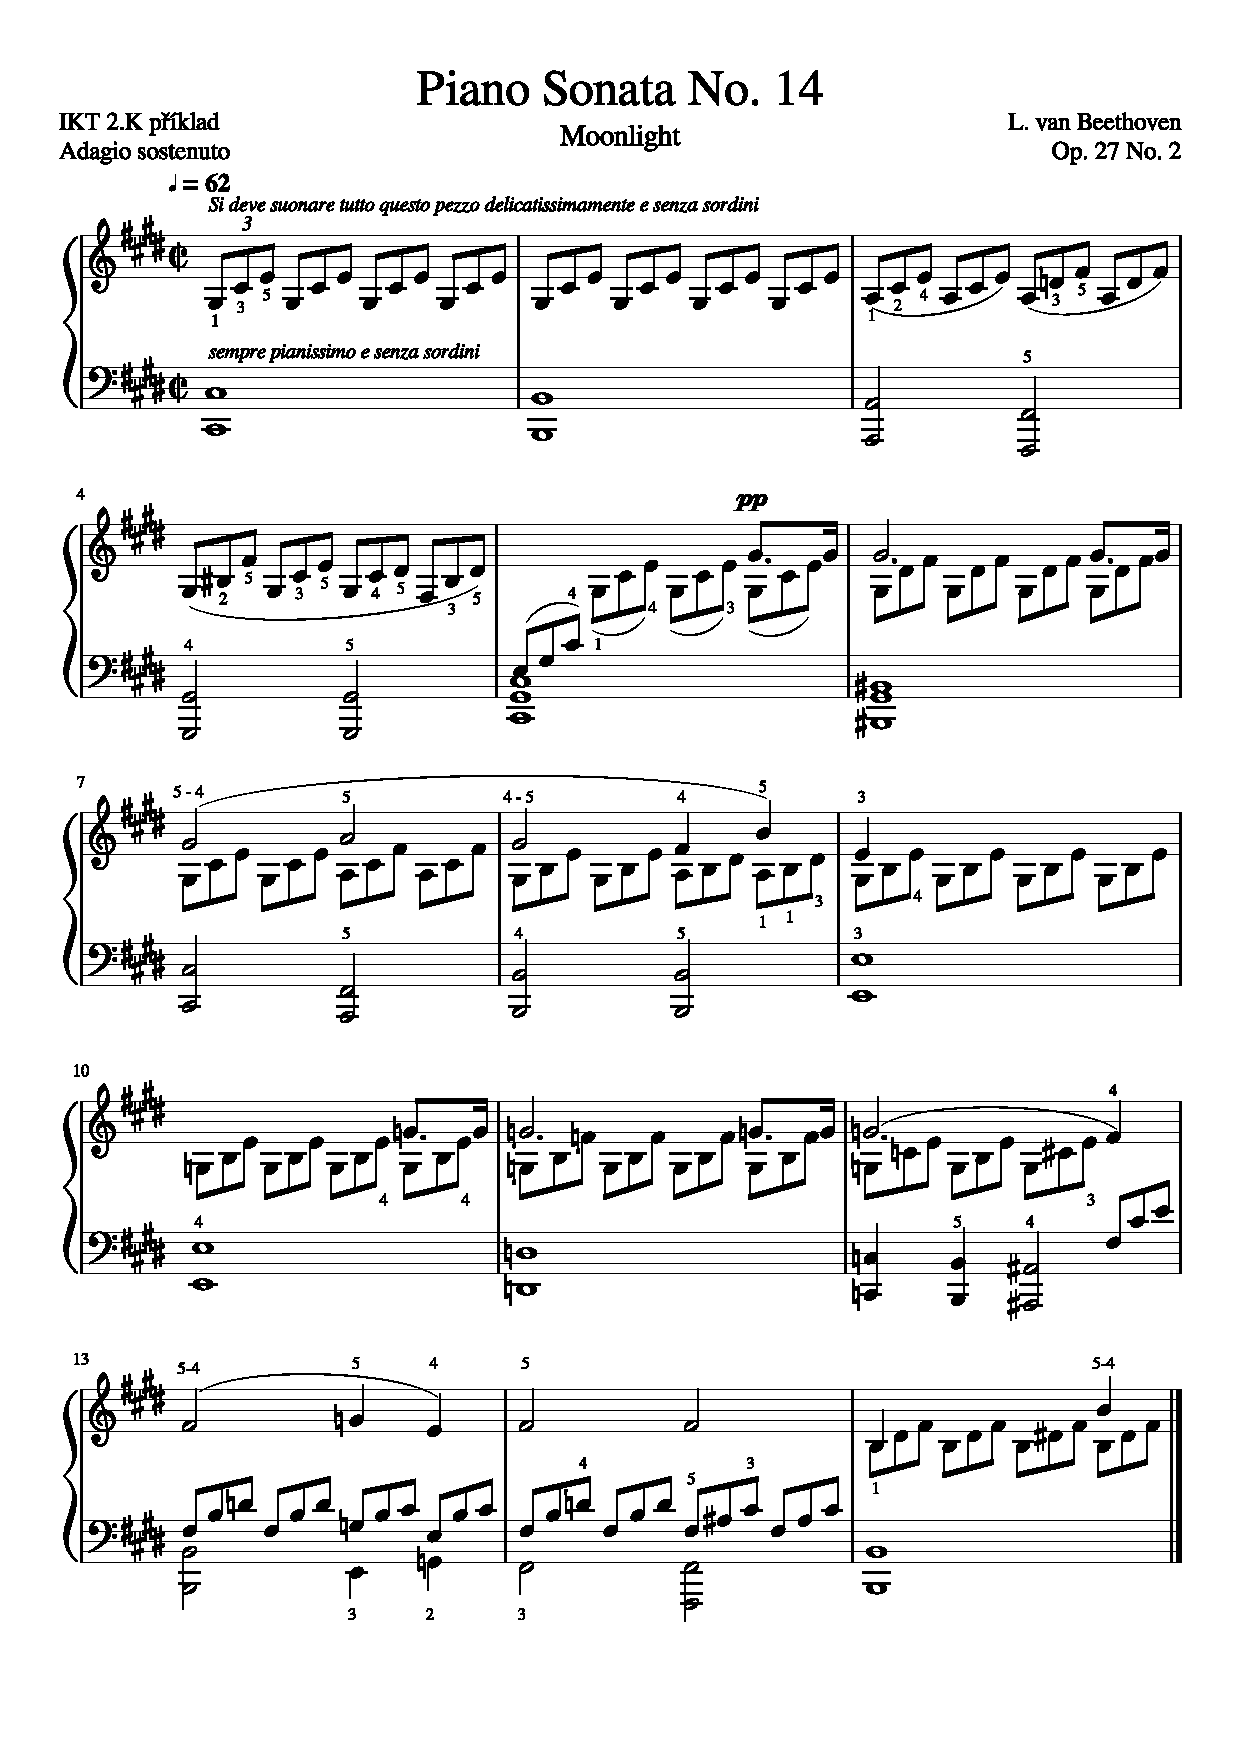
\includegraphics[width=\textwidth]{./obrazky/partitura-priklad.pdf}
    \end{center}
\end{figure}

\noindent
Přiložená partitura je příkladem naskenovaného notového materiálu o~výšce
větší než polovina stránky, o~kterém je pojednáváno ve~vlastním textu práce.

% ------------------------------------------------------------------------------

\end{appendices}


%-------------------------------------------------------------------------------
% KONEC DOKUMENTU
%-------------------------------------------------------------------------------

\end{document}
